\documentclass[aspectratio=169,10pt]{beamer}
\usepackage[UTF8]{ctex}\usepackage{booktabs,tabularx,amsmath,graphicx}
\usetheme{Madrid}\definecolor{navy}{HTML}{142B43}\definecolor{teal}{HTML}{168579}
\setbeamercolor{structure}{fg=navy}\setbeamercolor{frametitle}{bg=navy,fg=white}
\setbeamercolor{block title}{bg=teal,fg=white}\setbeamercolor{block body}{bg=teal!6}
\setbeamertemplate{navigation symbols}{}\setbeamertemplate{footline}{\leavevmode\hbox{\begin{beamercolorbox}[wd=.79\paperwidth,ht=2.5ex,dp=1ex,leftskip=1em]{author in head/foot}青序量化研究平台\quad CF2026 Project 1\end{beamercolorbox}\begin{beamercolorbox}[wd=.21\paperwidth,ht=2.5ex,dp=1ex,center]{date in head/foot}\insertframenumber/20\end{beamercolorbox}}}
\setbeamerfont{frametitle}{size=\large}\setbeamersize{text margin left=8mm,text margin right=8mm}
\begin{document}
\begin{frame}{青序量化研究平台}
\begin{block}{}从亏损案例到可复现的多因子研究\end{block}
\small\begin{itemize}
\item Computational Finance · Project 1
\item 1,000只历史股票，12个因子，5个候选
\item 最终评估：2025-01-02 至 2026-09-18
\end{itemize}
\note{这次展示包括平台本身和平台支持的策略研究。起点是一个真实的失败：原始动量长期亏损超过百分之八十。我们没有删除它，而是先核对数据和账本，再比较新的因子与风险组合。最后介绍验证期选出的策略，并说明它在哪些目标上达标、在哪些地方仍有限制。}
\end{frame}

\begin{frame}{Project 1 的核心是研究闭环}
\begin{block}{}基础80分与扩展20分，落实为可检查的证据\end{block}
\small\begin{itemize}
\item 数据：字段、复权、缺失、下载身份与哈希
\item 研究：因子、IC、分组、含费用回测、固定对照
\item 工程：同一核心供CLI和界面调用，保留测试与运行记录
\item 扩展：历史中性化、风险权重、部分成交、增量审计
\end{itemize}
\note{老师的要求没有规定必须达到某个收益或Sharpe。因此我们把正确性和复现放在第一位。每项要求都能从代码追到输出文件：例如因子分组保留形成时人数，成交文件保留实际金额和费用。扩展选择有验证证据的几项，不靠堆页面数。收益研究是平台能力的演示，同时接受失败结果。}
\end{frame}

\begin{frame}{原始动量的亏损超过费用拖累}
\begin{block}{}零费用独立重跑仍累计亏损75.16\%\end{block}
\centering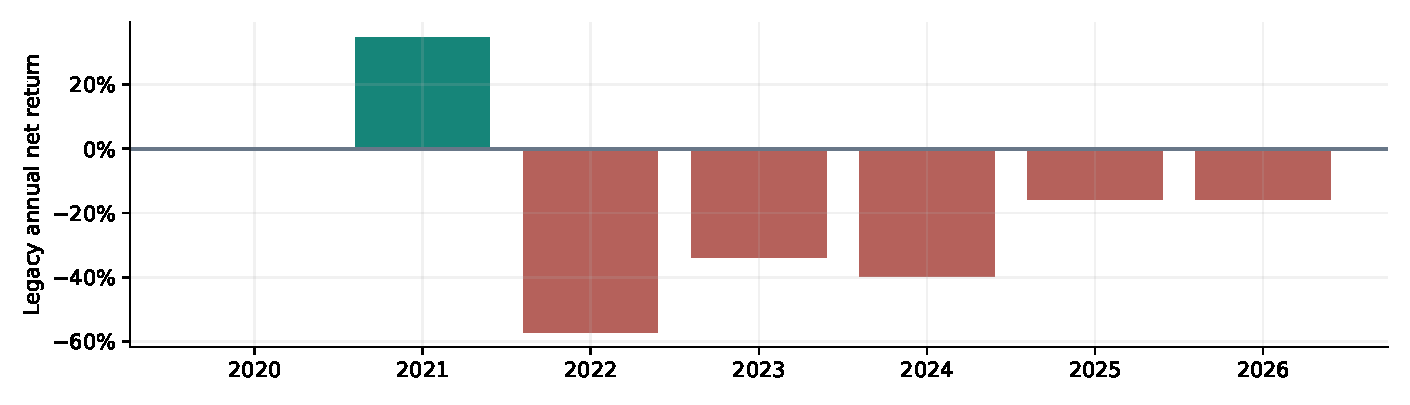
\includegraphics[width=.94\textwidth,height=.51\textheight,keepaspectratio]{figures/legacy.pdf}\par
\scriptsize\begin{itemize}
\item 原始扣费累计：$-$83.57\%，最大回撤89.83\%
\item 加回费用的同路径归因：$-$58.12\%
\item 零费用重跑会改变再投资路径，不能混为一谈
\end{itemize}
\note{原策略用二十日动量，每五个交易日调整前三十只股票。图里可以看到二零二二到二零二四年连续亏损。实际账本扣费亏损百分之八十三点五七，而真正将费用设为零再运行，仍亏损百分之七十五点一六。简单把累计费用加回净值，会得到另一条归因曲线。这个差异说明费用、仓位规模和后续盈亏有路径依赖。我们因此同时改进信号研究与组合构建。}
\end{frame}

\begin{frame}{分数与成交账本解耦}
\begin{block}{}新增模型输出同样的分数接口\end{block}
\small\begin{itemize}
\item 原始快照与质量检查
\item 因子/模型：日期$\times$资产分数
\item 组合模块：目标权重与现金
\item 成交模块：订单、成交、持仓、净值
\end{itemize}
\note{这里是可维护性的关键。模型只回答股票的相对分数，组合层决定多少资金投入，成交层决定订单实际完成多少。将来接入新因子或更复杂模型，不需要再写一套会计逻辑。命令行和界面调用相同函数。每次实验带上数据、参数和源码身份，避免出现界面显示一种口径、报告计算另一种口径。}
\end{frame}

\begin{frame}{1,656,599条日线具有明确来源}
\begin{block}{}固定2019年末股票池，保留后来缺失的成员\end{block}
\begin{center}\small\begin{tabularx}{.96\textwidth}{lX}\toprule
项目 & 结果\\\midrule
资产 / 交易日 & 1,000 / 1,690\\
日线重复键 / 异常剔除 & 0 / 0\\
缺失网格 / 缺限制价 & 33,401 / 48\\
每日估值记录 & 1,656,599\\
\bottomrule\end{tabularx}\end{center}
\small\begin{itemize}
\item 价格区间：2019-10-08 至 2026-09-18
\item 57,389条财务指标，1,432条历史行业区间
\item 原行情3,006个文件、新研究2,073个文件哈希核验
\item 固定池不含后续IPO，也不代表全A股
\end{itemize}
\note{股票池在二零一九年末按当时成交额选取，收益研究从之后开始。我们没有拿今天还上市的股票倒推历史。完整网格有三万三千多条缺失，缺失会影响因子、成交和估值，所以分别处理并计数。补充每日估值、公告和历史行业后，整体本地存储约一点六三GB。最重要的边界是固定池的选择偏差和厂商事后修订，它们不会因为数据量大而自动消失。}
\end{frame}

\begin{frame}{时间分割先于结果}
\begin{block}{}2023–2024验证选择，2025年后只作评估\end{block}
\small\begin{itemize}
\item 2020–2022训练：653,622个有效样本
\item 清除标签退出日跨入2023年的训练观测
\item 财报严格晚于公告日使用
\item 原动量全期已被观察：不称完全未知的盲测
\end{itemize}
\note{这里需要区分报告期和信息可用时间。年度财报不能在十二月三十一日就拿来预测，要等公告之后。标签是明天开盘买入、二十个交易日后开盘退出的收益，边界附近的训练标签会跨入验证期，所以需要清除。最终候选只依据验证段选择。不过我们此前确实已经看过原始动量在全区间的表现，因此必须承认最终段并非完全未知的盲测。}
\end{frame}

\begin{frame}{12个因子构成可解释的基线}
\begin{block}{}既保留防御与价值，也保留表现不佳的方向\end{block}
\begin{center}\small\begin{tabularx}{.96\textwidth}{lX}\toprule
类别 & 因子\\\midrule
趋势 / 反转 & 跳月动量、5日反转、20日均线趋势\\
风险 / 量价 & 低波动、低振幅、量能变化、流动性、低换手\\
价值 / 分红 & 盈利收益率、账面市值比、股息率\\
质量 & 最新已公告年度ROE\\
\bottomrule\end{tabularx}\end{center}
\small\begin{itemize}
\item 同日横截面统一方向与尺度
\item 至少10个因子有效，其余标准化缺值取中性值0
\item 完整因子卡列出字段、窗口与失败情形
\end{itemize}
\note{这十二个因子并不是十二个独立的信息源。低波动和低振幅就可能高度相关。它们覆盖中期趋势、短期反转、风险、量价、价值和盈利质量。我们提前固定符号，在最终期IC为负时也不直接翻转。参考了Qlib的量价表达，但没有声称完整实现Alpha158。后续需要以独立验证证明新增因子提供额外信息。}
\end{frame}

\begin{frame}{中性化控制已知风格暴露}
\begin{block}{}每个形成日单独处理，避免全样本标准化\end{block}
\[z_{i,t}=\alpha_{g(i),t}+\beta_t\log MV_{i,t}+\epsilon_{i,t}\]
\small\begin{itemize}
\item 1\% / 99\%截尾，再用当日样本均值和标准差标准化
\item 回归当时有效的行业虚拟变量与对数市值
\item 残差重新标准化，检查行业均值与市值正交
\item UNKNOWN单独成组，历史分类不反填
\end{itemize}
\note{中性化可以解释为剥离行业和市值能解释的部分。我们先在每个行业内将因子和对数市值去均值，再回归得到残差，这与包含行业虚拟变量的OLS一致。测试检查残差的行业均值和与市值的内积。需要注意，中性化不等于增加预测信息；如果原先有用的风格收益被去掉，实际收益可能下降。因此同时保留标准化和中性化的等权基线进行对照。}
\end{frame}

\begin{frame}{小型神经网络是一个对照候选}
\begin{block}{}输入是表格因子，采用MLP回归相对收益秩\end{block}
\small\begin{itemize}
\item Ridge：线性、正则化、容易解释
\item LightGBM：固定250棵树与受限树深
\item MLP：12 $\to$ 32 $\to$ 16 $\to$ 1，ReLU，固定8轮
\item 相同组合与费用评估，MLP未声称已收敛
\end{itemize}
\note{同学建议预测涨跌并使用CNN。我们的判断是，涨跌标签会丢失收益幅度和横截面排序信息，而任意排列的十二个因子不具备图像像素那样的邻接结构。因此使用小型全连接网络，目标是当日未来收益的百分位秩。三个学习模型都只用训练区间，固定参数和随机种子。八轮MLP没有收敛，结果只能代表这次受限配置，不能据此否定神经网络。}
\end{frame}

\begin{frame}{每笔费用只对应实际成交}
\begin{block}{}收盘形成信号，最早下一开盘执行\end{block}
\[fee_t=0.001B_t+0.0015S_t,\quad NAV_t=Cash_t+\sum_i q_{i,t}P_{i,t}\]
\small\begin{itemize}
\item 买10bp、卖15bp，按实际成交额计提
\item 涨跌停、缺报价和现金约束可阻止或缩减成交
\item 此前20日平均成交额的1\%限制单资产成交预算
\item 独立重建现金、单位余额、每日净值与费用
\end{itemize}
\note{假设今天收盘形成信号，明天开盘才可以交易。开盘先处理卖单，再根据实际可用现金处理买单，不能假设被停牌阻挡的卖单已经收到资金。流动性预算只用之前二十日成交额，不能用今天收盘后才知道的成交量。所有拒单和部分成交都留下状态，未成交部分不收费。研究单位是连续可分的复权单位，这仍与整手实盘、真实分红现金和盘口排队存在差别。}
\end{frame}

\begin{frame}{风险预算让组合可以持有现金}
\begin{block}{}降低回撤，同时接受上涨参与度下降\end{block}
\small\begin{itemize}
\item 每20个交易日调仓，50只目标持仓，前70名保留缓冲
\item 单股目标$\leq$4\%，行业目标$\leq$25\%，股票预算$\leq$90\%
\item 年化波动目标12\%，过去60日估计风险
\item 沪深300低于120日均线时，股票预算乘0.25
\end{itemize}
\note{我们允许现金，因此不必在风险很高的时候仍然满仓。组合按低波动倾斜并限制单股和行业目标，再根据估计波动率和市场趋势缩减总仓位。目标上限是在形成时成立，成交受阻和后续价格变化会使实际权重漂移。波动率和最大回撤也不是硬保证。这一策略最终平均持有约一半现金，所以应当预期它在上涨市场中可能落后指数。}
\end{frame}

\begin{frame}{验证期选择了标准化多因子}
\begin{block}{}年化5.84\%，最大回撤7.20\%，符合预先选择规则\end{block}
\centering
\includegraphics[width=.94\textwidth,height=.51\textheight,keepaspectratio]{figures/validation.pdf}\par
\note{这张图是唯一用于选择提交策略的阶段。我们优先考虑正年化且回撤不超过百分之二十的候选，再比较年化收益除以回撤。标准化多因子最优。中性化基线和MLP有很小的正收益，Ridge较好但回撤更高，LightGBM在这段是负收益。没有因为模型更复杂就给它额外优先级。选择结果先落盘，再运行下一阶段。}
\end{frame}

\begin{frame}{最终期保留全部候选结果}
\begin{block}{}LightGBM后续较强，仍不替换验证期预选策略\end{block}
\centering
\includegraphics[width=.94\textwidth,height=.51\textheight,keepaspectratio]{figures/test_models.pdf}\par
\note{最终期的排序与验证期明显不同。LightGBM年化超过百分之十三，如果只展示这张表，很容易事后挑出它当冠军。但这样做会把测试期变成新的验证期。我们保留验证选出的标准化多因子，其他模型作为后续研究线索。表里也能看到复杂模型更高的换手和费用。以后要证明LightGBM值得升级，需要新的未观察数据或严格滚动验证。}
\end{frame}

\begin{frame}{预选策略达到CPI目标，尚未战胜指数}
\begin{block}{}累计净收益6.12\%，年化3.65\%，最大回撤7.01\%\end{block}
\centering
\includegraphics[width=.94\textwidth,height=.51\textheight,keepaspectratio]{figures/nav.pdf}\par
\scriptsize\begin{itemize}
\item 共同完整月份2025/02–2026/08：策略7.02\%，CPI 0.69\%
\item 沪深300为未扣复制成本的价格指数；现金按零利息
\end{itemize}
{\tiny 本页展示完整417日净值；PowerPoint版每5个交易日取点。}
\note{这张净值图应与风险一起看。预选策略累计收益约百分之六点一二，最大回撤约百分之七点零一。同期价格指数收益更高，回撤也更高。购买力比较使用完全相同的十九个完整月份：策略约百分之七点零二，CPI约百分之零点六九。为什么与累计六点一二不同？因为完整月份比较剔除了起始月份和最后一个不完整月份。我们不会把不同区间的数字直接放在一起作结论。}
\end{frame}

\begin{frame}{同一分数下，风险控制减少回撤}
\begin{block}{}双倍费用下年化约3.18\%，回撤约7.24\%\end{block}
\centering
\includegraphics[width=.94\textwidth,height=.51\textheight,keepaspectratio]{figures/controls.pdf}\par
\scriptsize\begin{itemize}
\item 满仓等权：年化4.81\%，回撤13.12\%
\item 风险组合：年化3.65\%，回撤7.01\%
\item 整套组合模块对照，不能单独归因于趋势过滤
\end{itemize}
\note{这组比较固定股票分数，改变组合模块。满仓等权的收益稍高，但回撤接近风险组合的两倍。双倍费用实验固定其他规则，只提高买卖费率，仍保持正收益，体现较低换手的作用。零费用是完整重跑，与之前费用加回归因区分开。需要坦诚的是，满仓等权同时取消了缓冲、逆波动和行业限制，所以只能解释整套组合设计的净作用。}
\end{frame}

\begin{frame}{因子诊断同时保留负结果}
\begin{block}{}878个形成日，逐日横截面IC与20日标签\end{block}
\centering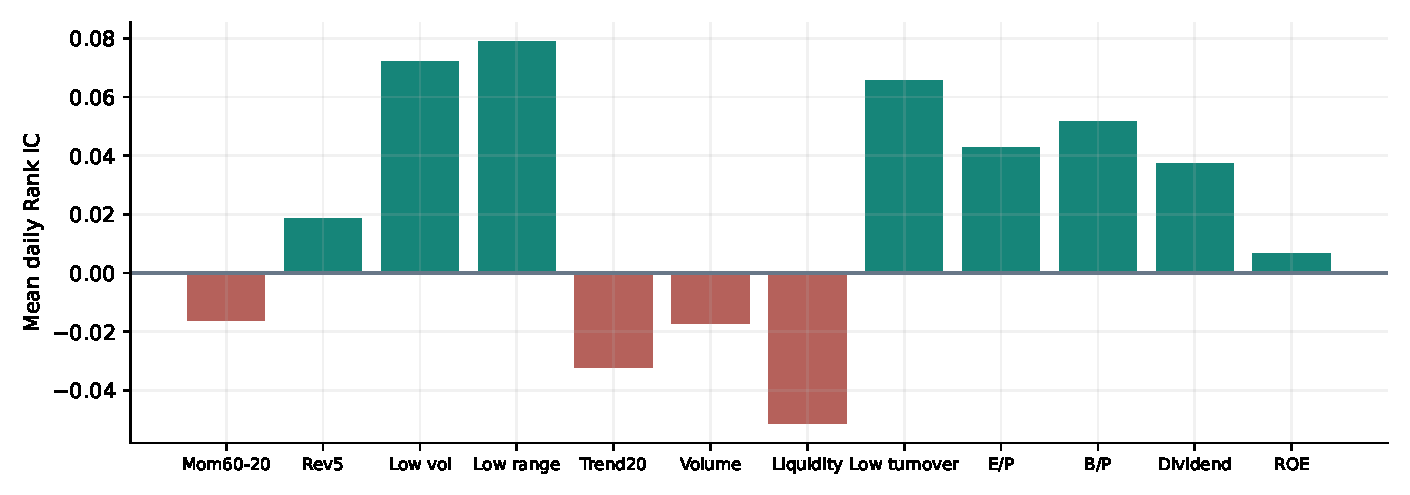
\includegraphics[width=.94\textwidth,height=.51\textheight,keepaspectratio]{figures/factor_ic.pdf}\par
\scriptsize\begin{itemize}
\item 低波动与低振幅较强，仍需检查信息冗余
\item 先形成五组，再匹配未来标签；不重新分组
\item 重叠20日收益均值不连乘成净值，不声称显著性
\end{itemize}
\note{这里展示中性化因子的平均Rank IC。低波动、低振幅和低换手较好，流动性和均线趋势为负。每一天先跨股票计算相关，再沿时间汇总；这与把全部股票日混在一起算一次相关不同。分组也先依据当日分数固定，再统计未来收益和缺失人数。因为标签重叠，相邻二十日收益并不独立，因此这些平均值属于诊断，不能直接称为可交易收益或显著alpha。}
\end{frame}

\begin{frame}{现场演示：从结论追到证据}
\begin{block}{}两分钟完成研究页、因子诊断与回测核验\end{block}
\small\begin{itemize}
\item 策略研究：确认预选名称、日期、CPI共同月份
\item 模型对照：解释为什么没有选择后续冠军
\item 因子诊断：查看公式、覆盖与形成/有效人数
\item 回测实验：用预热样本运行并查看账本通过状态
\end{itemize}
\note{现场先打开默认策略研究页，读出区间和预选模型，指出CPI使用共同完整月份。然后切换模型对照解释验证选择，进入因子诊断选一个正IC和一个负IC因子，看定义及有效人数。最后切到交互回测，使用事先预热的样本提交一次，展示账本核验通过和交易导出。若教室网络或页面有问题，直接用已保存的截图和PDF继续；现场不下载数据，也不重新训练模型。}
\end{frame}

\begin{frame}{平台已形成可复现的研究基础}
\begin{block}{}收益目标有条件达成，风险与数据边界继续保留\end{block}
\small\begin{itemize}
\item 达到：扣费后超过同期CPI，历史回撤低于20\%
\item 未达到：年化5\%–8\%的更高期望及战胜市场
\item 边界：固定池、财报修订、复权单位、风险目标漂移
\item 下一步：新的滚动验证区间与更真实的成交模型
\end{itemize}
\note{我们的主要贡献是把数据、因子、执行、统计和证据连接起来。策略在这段历史达到CPI目标，回撤也低于事先设定的目标，但更高收益期望没有达到。对已实现收益做分块重采样得到的区间也包含负年化，这提示我们不能保证未来回报。后续可以扩展滚动训练和Qlib因子，但每一步都应该在新的验证条件下进行，而不是继续调整这段最终区间来追求更漂亮的数字。}
\end{frame}

\begin{frame}{备份：绩效与购买力口径}
\begin{block}{}期初净值参与第一日收益与最大回撤\end{block}
\[R_{real}=\frac{1+R_{strategy}}{1+\pi_{CPI}}-1\]
\small\begin{itemize}
\item 年化： (NAV末 / NAV初)\textasciicircum{}(252 / 交易日数) $-$ 1
\item Sharpe：$\sqrt{252}$ $\times$ 日超额均值 / 日超额样本标准差
\item CPI累计：逐月(1 + 月环比)相乘 $-$ 1
\item 实际收益：(1 + 策略收益) / (1 + CPI累计) $-$ 1
\end{itemize}
\note{回答口径问题时使用。无风险年利率默认零，日标准差ddof为一；零波动Sharpe记缺失。回撤高水位包含初始资金。CPI同比没有参与连乘。价差分组没有冒充可执行多空策略，费用加回也没有冒充无费用独立重跑。}
\end{frame}

\begin{frame}{备份：来源与答辩问题}
\begin{block}{}复杂模型、中性化与平台正确性可以分别讨论\end{block}
\small\begin{itemize}
\item 为什么不用CNN？因子顺序无天然邻接，MLP更直接
\item 为什么不选LightGBM？验证期规则已经固定
\item Qlib复现了吗？参考工作流与表达，未完整复制Alpha158
\item 主要来源：课程课件、Tushare、Qlib、CogAlpha、sklearn
\end{itemize}
\note{来源：课程CF2026\_Project1.pdf共十九页；Tushare官方日线、复权、估值、财务和行业接口；Microsoft Qlib官方仓库及Alpha158/LightGBM示例；Liu等CogAlpha论文v4。若问满分，回答我们按所有基础项和有证据扩展逐项准备，评分由老师判断。若问能否实盘，回答还需整手、分红现金、手续费历史和微观成交等验证。}
\end{frame}
\end{document}